W poprzednich rozdziałach zidentyfikowano problem, kontekst oraz plan projektowy – teraz nadszedł moment, by przedstawić odpowiedź: architekturę systemu, który usprawni zarządzanie danymi i automatyzację procesów. Ale dlaczego właśnie taką? Co sprawiło, że przyjęto konkretne założenia, a inne odrzucono? Jak przebiegał proces decyzyjny, który doprowadził do ostatecznej formy rozwiązania?

Projektowanie architektury to nie tylko kwestia technicznych decyzji – to poszukiwanie balansu między funkcjonalnością, wydajnością i bezpieczeństwem, a także uwzględnienie ograniczeń i przyszłych potrzeb użytkowników. W tym rozdziale przedstawione zostaną kolejne etapy tego procesu, począwszy od analizy wymagań, poprzez wybór kluczowych komponentów, aż po podejmowanie decyzji architektonicznych, które zdeterminowały finalną formę systemu.

\section{Definicja wymagań funkcjonalnych i niefunkcjonalnych}
Po zrozumieniu problemu i podstawowych założeń, określono wymagania funkcjonalne i niefunkcjonalne dla systemu automatyzacji danych Sciencepreneurs Club. System miał przede wszystkim umożliwić automatyzację procesu rejestracji uczestników i usprawnić zarządzanie danymi w \gls{cinn}.

Funkcjonalnie system został zaprojektowany, aby realizować rejestrację użytkowników poprzez formularz Microsoft Forms, gdzie dane są automatycznie przetwarzane i zapisywane w centralnej bazie \gls{excel}. Świadomie zrezygnowano z ręcznego dopisywania uczestników, redukując tym samym ryzyko pomyłek i utraty danych. System zapewnia zarządzanie danymi w dynamicznej strukturze, umożliwiającej analizę i raportowanie, a także analizę frekwencji poprzez przetwarzanie danych rejestracyjnych przez \gls{powerquery}.

W zakresie wymagań niefunkcjonalnych priorytetem stały się efektywność operacyjna i bezpieczeństwo danych.

Proces rejestracji działa autonomicznie w tle, eliminując konieczność bieżącej ingerencji administratora. System automatycznie przetwarza dane od momentu wypełnienia formularza do wprowadzenia ich do bazy. Choć przygotowanie nowej edycji wymaga rozszerzonej konfiguracji przez administratora, rezultatem jest w pełni zautomatyzowany proces niewymagający bieżących interwencji, co zapewnia wysoką efektywność operacyjną w długiej perspektywie.

System uwzględnia aspekty ochrony danych osobowych - wszystkie informacje uczestników są przechowywane w zasobach \gls{inin} zgodnie z polityką bezpieczeństwa wchodzących w \gls{microsoft365}. Rozwiązanie korzysta z wielowarstwowej architektury zabezpieczeń, która obejmuje zarówno mechanizmy na poziomie platformy, jak i specyficzne zabezpieczenia implementowane na poziomie poszczególnych komponentów. 

Również niezawodność jest jednym z kluczowych kryteriów wymagań niefunkcjonalnych. System bazuje na sprawdzonej infrastrukturze \gls{microsoft365}, co gwarantuje wysoką dostępność zgodnie z umową \gls{sla} na poziomie 99,9\%. W przypadku potrzeby przywrócenia danych, historia wersji plików przechowywana w \gls{sharepoint} umożliwia bezpieczne odtworzenie wcześniejszych zapisów. 

Dzięki przyjętej architekturze, system jest elastyczny i nie wymaga wyłączania podczas aktualizacji – wszelkie zmiany wprowadzane są poprzez duplikację i edycję istniejących elementów, co eliminuje ryzyko przerwy w działaniu w trakcie trwającej rejestracji. 

\section{Decyzje Technologiczne}
Projektowanie systemu zarządzania danymi dla \gls{cinn} było nie tylko kwestią doboru odpowiednich narzędzi, lecz także strategiczną decyzją, która miała kluczowe konsekwencje dla jego wdrożenia i późniejszego utrzymania. Wybór technologii stanowił element długotrwałych rozważań, w których uwzględniano zarówno potrzeby organizacyjne, jak i istniejące ograniczenia infrastrukturalne.

Już na wczesnym etapie rozważań pojawiła się idea stworzenia systemu opartego na relacyjnej bazie danych \gls{sql}. Logika tego rozwiązania była oczywista – umożliwiałoby ono lepszą integralność danych, automatyzację procesów, a także zapewniało wyższy poziom bezpieczeństwa i łatwość zarządzania kopiami zapasowymi. Dodatkowo, w perspektywie długoterminowej, migracja na SQL mogłaby uprościć dalszą automatyzację i integrację z innymi systemami uczelnianymi. Jednak decyzja ta nie należała wyłącznie do zespołu projektowego. Kluczowe było stanowisko kierownictwa \gls{inin}, które – analizując koszty i realia organizacyjne – uznało, że wdrożenie nowego systemu bazodanowego byłoby zbyt dużym wyzwaniem w kontekście bieżących zmian technologicznych.

\gls{inin} znajdował się w fazie stopniowej migracji do chmury, a większość danych wciąż była przechowywana w klasycznej strukturze folderów on-prem. Implementacja \gls{sql} oznaczałaby konieczność restrukturyzacji istniejących procesów, co wiązałoby się z dodatkowymi kosztami operacyjnymi oraz koniecznością zapewnienia specjalistycznej obsługi. W tym kontekście uzasadnionym wyborem stało się pozostanie przy rozwiązaniach już stosowanych w organizacji – zwłaszcza tych dostępnych w ramach licencji \gls{microsoft365}.

Alternatywne podejście, które ostatecznie przyjęto, zakładało wykorzystanie \gls{excel} jako głównej bazy danych, przy jednoczesnym zastosowaniu \gls{powerautomate} i \gls{powerquery} do automatyzacji procesów. Dzięki temu można było uniknąć konieczności kosztownej migracji, a jednocześnie zapewnić sprawną organizację danych i ich analizę w ramach istniejącej infrastruktury. Co więcej, to rozwiązanie pozwalało na szybkie wdrożenie systemu bez potrzeby angażowania dodatkowych zasobów \gls{it} oraz umożliwiało łatwe zarządzanie przez osoby nieposiadające specjalistycznej wiedzy technicznej.

Decyzja ta nie była wolna od kompromisów. \gls{excel}, mimo swojej elastyczności, nie jest narzędziem stworzonym do obsługi dużych zbiorów danych, co rodziło pytania o skalowalność i wydajność systemu w przypadku dalszego rozwoju projektu. Niemniej jednak, w warunkach \gls{inin}, gdzie priorytetem było szybkie wdrożenie i utrzymanie zgodności z obecnym środowiskiem \gls{it}, wybór ten okazał się najbardziej praktyczny. W przyszłości możliwe będzie ponowne rozważenie implementacji bazy danych \gls{sql}.
Tym samym, proces decyzyjny nie polegał jedynie na wyborze technologii, lecz na znalezieniu rozwiązania najbardziej optymalnego w kontekście realiów organizacyjnych. Elastyczność w podejściu do wyboru technologii jest kluczowym aspektem projektowania rozwiązań dla instytucji przechodzących transformację cyfrową.

\section{Architektura zabezpieczeń}

Architektura zabezpieczeń systemu Sciencepreneurs Club implementuje wielowarstwowe podejście do ochrony danych, wykorzystując zarówno mechanizmy platformy \gls{microsoft365}, jak i specyficzne zabezpieczenia na poziomie poszczególnych komponentów. Łącząc uwierzytelnianie uczelniane, autoryzację opartą o role, szyfrowanie danych, historię wersji i automatyczne kopie zapasowe, system zapewnia solidną ochronę przed typowymi zagrożeniami.

\begin{figure}[!hb]
	\centering 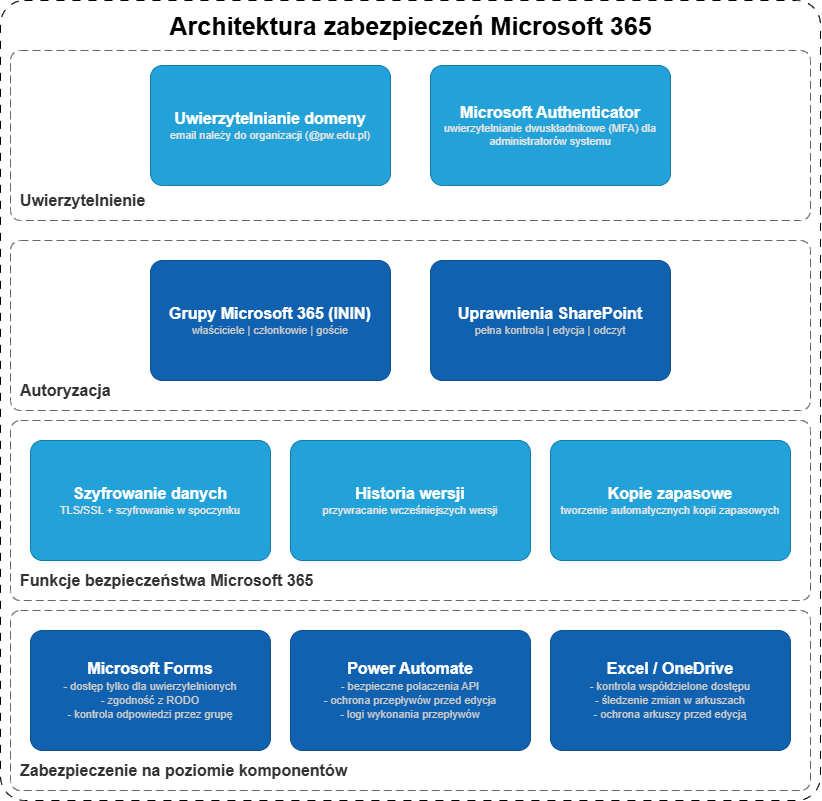
\includegraphics[width=0.85\linewidth]{rysunki/ArchitekturaZabezpieczen.png}
	\caption{Architektura zabezpieczeń systemu automatyzacji baz danych dla Sciencepreneurs Club w, źródło: opracowanie własne}
\end{figure}

Uwierzytelnianie stanowi pierwszą linię obrony w architekturze bezpieczeństwa systemu, zapewniając weryfikację tożsamości wszystkich użytkowników wchodzących w interakcję z aplikacją. Fundamentem bezpieczeństwa systemu jest \gls{entraid}. Ten centralny system zarządzania tożsamościami pozwala użytkownikom logować się do zasobów przy użyciu kont uczelnianych z domeną @pw.edu.pl, niezależnie od urządzenia, z którego korzystają. \gls{entraid} obejmuje również integrację z aplikacją Microsoft Authenticator, która korzysta z funkcjonalności \gls{mfa}. Jest to szczególnie istotne dla administratorów systemu, zapewniając dodatkową ochronę przed nieautoryzowanym dostępem nawet w przypadku kompromitacji hasła.

\begin{figure}[!hb]
	\centering 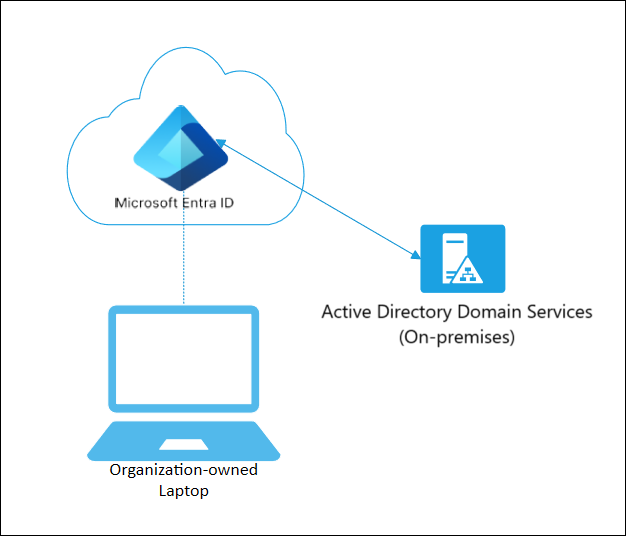
\includegraphics[width=0.7\linewidth]{rysunki/entraid.png}
	\caption{Autentykacja dostępu za pomocą \gls{entraid} , źródło: \cite{microsoft_entra_devices_2025}}
\end{figure}

Kluczową zaletą architektury opartej na \gls{entraid} jest uniezależnienie dostępu od konkretnego sprzętu. Członkowie zespołu mogą korzystać z dowolnego komputera lub urządzenia mobilnego, mając pewność, że po uwierzytelnieniu uzyskają dostęp do wszystkich zasobów grupy przechowywanych w chmurze. W przypadku awarii sprzętu, zgubienia urządzenia lub wymiany komputera, nie ma potrzeby rekonfiguracji dostępów – wszystkie uprawnienia są powiązane z kontem użytkownika w \gls{entraid}, a nie z fizycznym urządzeniem. Eliminuje to przestoje związane z problemami technicznymi i zapewnia ciągłość pracy.
\gls{entraid}  integruje się z systemami zarządzania cyklem życia kont na uczelni, co gwarantuje automatyczną dezaktywację dostępu dla osób, które przestały być związane z \gls{pw}. \cite{microsoft_entra_devices_2025} 

Po pomyślnym uwierzytelnieniu, warstwa autoryzacji definiuje precyzyjny zakres dostępu użytkownika do konkretnych zasobów i funkcji. System implementuje model kontroli dostępu oparty o role poprzez grupy \gls{microsoft365}. \cite{Microsoft365Groups2025} Podstawą organizacji uprawnień jest grupa \texttt{"Inkubator\_PW"} z trzema poziomami dostępu. 
Właściciele posiadają pełen dostęp administracyjny do wszystkich komponentów systemu. Członkowie – ze standardowym dostępem operacyjnym mają wgląd do przeglądania i ograniczonej edycji. Na najniższym poziomie są goście, z dostępem tylko do odczytu wybranych zasobów. Uzupełnieniem są szczegółowe uprawnienia \gls{sharepoint} na poziomie repozytorium dokumentów (pełna kontrola, edycja, odczyt), zapewniające precyzyjną kontrolę zgodną z zasadą minimalnych uprawnień.

Platforma \gls{microsoft365} oferuje szereg wbudowanych mechanizmów bezpieczeństwa wykorzystywanych w systemie. Szyfrowanie danych obejmuje zarówno szyfrowanie transmisji (\gls{tls}/\gls{ssl}) jak i szyfrowanie danych w spoczynku. \cite{microsoft_encryption_2024} Historia wersji zapewnia automatyczne śledzenie zmian w dokumentach z możliwością przywracania wcześniejszych wersji. Dodatkowo system korzysta z automatycznych kopii zapasowych.

Każdy z trzech głównych komponentów systemu implementuje dodatkowe mechanizmy bezpieczeństwa. \gls{forms} wprowadza implementację klauzul zgodnych z \gls{rodo}. Power Automate zapewnia bezpieczne połączenia \gls{api} z uwierzytelnianiem ustandaryzowanym wewnątrz środowiska \gls{microsoft365}. \cite{microsoft_encryption_2024}. \gls{excel} i \gls{onedrive} dostarczają kontrolę współdzielonego dostępu, śledzenie zmian w arkuszach, selektywną ochronę arkuszy i zakresów komórek przed edycją oraz zdefiniowane role dostępu. \cite{microsoft_office_versions_2025} \cite{microsoft_excel_blocking_2025}

Architektura zabezpieczeń systemu Sciencepreneurs Club stanowi wielowarstwowy system ochrony, który łączy mechanizmy \gls{entraid}, kontroli dostępu bazującej na rolach, szyfrowania danych oraz specyficznych zabezpieczeń komponentowych. Takie podejście zapewnia odpowiedni poziom bezpieczeństwa przy jednoczesnym zachowaniu elastyczności i użyteczności systemu.

\section{Diagram czynności}

Proces rejestracji uczestników wydarzeń opiera się na zautomatyzowanym systemie, który minimalizuje konieczność ręcznej obsługi zgłoszeń. Każda nowa edycja wydarzenia rozpoczyna się od wykonania przez administratora zestawu powtarzalnych czynności przygotowawczych. Zadania, które nadal wymagają manualnej interwencji, zostały precyzyjnie zmapowane, co umożliwia ich przyszłą automatyzację w kolejnych etapach rozwoju systemu.

\newpage
\begin{figure}[!hb]
	\centering 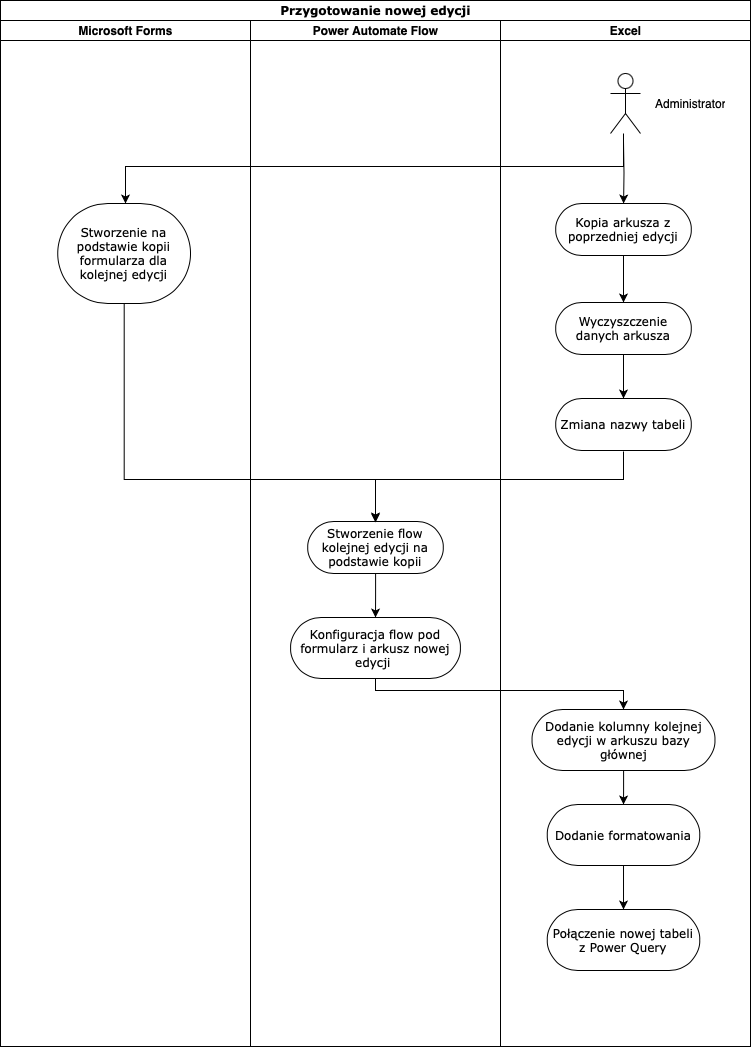
\includegraphics[width=0.85\linewidth]{rysunki/przygotowanie.png}
	\caption{Przygotowanie na kolejną edycję - administrator, źródło: opracowanie własne }
\end{figure}

Każda nowa edycja wydarzenia wymaga uprzedniego przygotowania przez administratora. Proces ten rozpoczyna się od organizacji bazy danych, co obejmuje skopiowanie arkusza z poprzedniej edycji, usunięcie wcześniejszych wpisów, nadanie nowej nazwy oraz dostosowanie istniejących formuł. Równocześnie tworzony jest nowy formularz rejestracyjny na podstawie wzorca z poprzedniego wydarzenia, z uwzględnieniem zmiany nazwy, prelegenta, tematu oraz terminu. Następnie konieczna jest aktualizacja przepływu pracy w \gls{powerautomate}, polegająca na skopiowaniu istniejącego procesu, dostosowaniu nazwy oraz podpięciu nowego formularza i tabeli w bazie danych. Ostatnim etapem konfiguracji jest uaktualnienie raportów poprzez dodanie nowej edycji do głównej bazy danych, wprowadzenie reguł formatowania dla nowej daty oraz aktualizację źródeł w \gls{powerquery}. Po wykonaniu tych kroków dalszy przebieg rejestracji odbywa się bez konieczności nadzoru ze strony administratora – wszystkie zgłoszenia są automatycznie zapisywane i przetwarzane.

\begin{figure}[!hb]
	\centering 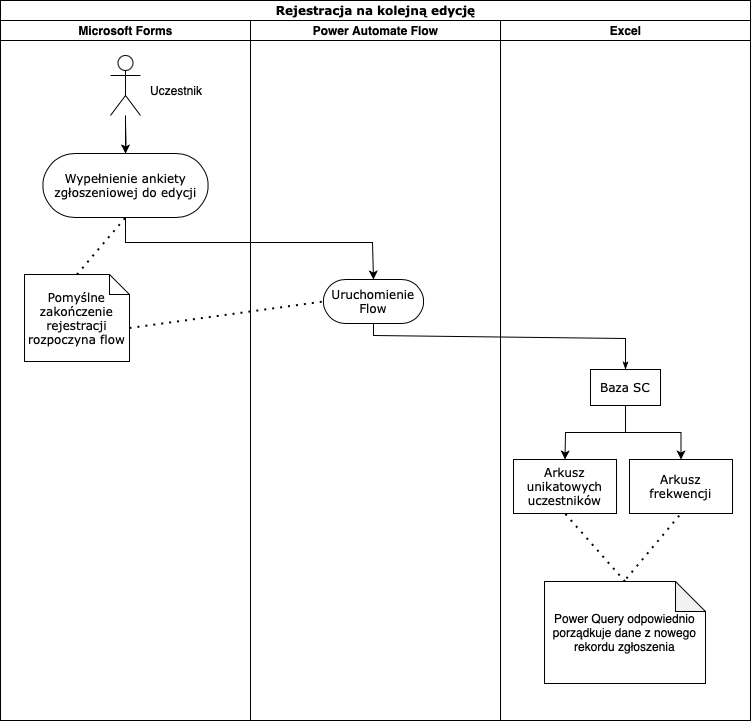
\includegraphics[width=0.85\linewidth]{rysunki/registration.png}
	\caption{Rejestracja na kolejną edycję - uczestnik, źródło: opracowanie własne}
\end{figure}

Uczestnicy otrzymują link do formularza rejestracyjnego stworzonego w Microsoft Forms, gdzie podają podstawowe informacje, takie jak imię, nazwisko, adres e-mail oraz temat wydarzenia. Po przesłaniu formularza dane są automatycznie przekazywane do centralnej bazy danych w arkuszu Excel za pośrednictwem przepływu pracy skonfigurowanego w \gls{powerautomate}. Dzięki temu administrator nie musi podejmować żadnych dodatkowych działań – zgłoszenia są zapisywane w bazie w sposób całkowicie zautomatyzowany.

\section{Architektura systemu}
Architektura systemu zarządzania uczestnikami Sciencepreneurs Club została zaprojektowana zgodnie z podejściem warstwowym, gdzie każdy komponent odpowiada za ściśle określony obszar funkcjonalny. Jednocześnie, dzięki wykorzystaniu platformy \gls{microsoft365}, zapewniono wysoki poziom integracji między poszczególnymi elementami.

\begin{figure}[!ht]
\centering
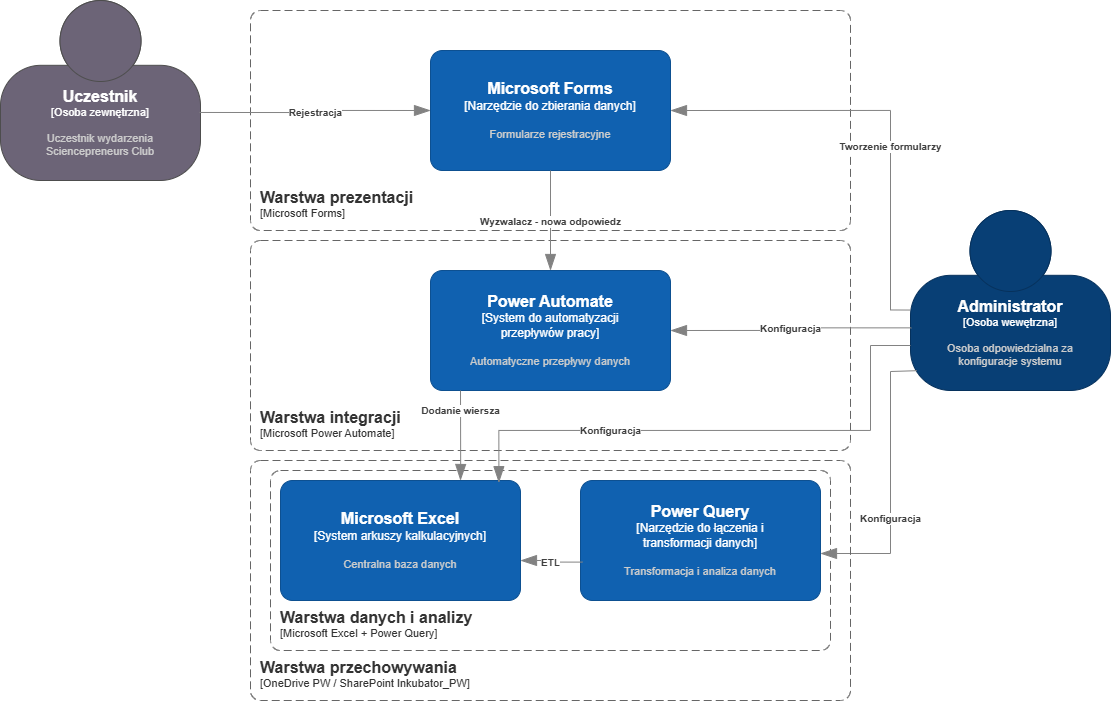
\includegraphics[width=1\linewidth]{rysunki/ArchitekturaSystemu.PNG}
\caption{Architektura systemu zarządzania uczestnikami Sciencepreneurs Club, żródło: opracowanie własne}
\label{fig}
\end{figure}

System charakteryzuje się architekturą warstwową, gdzie:

\begin{itemize}
\item \textbf{Warstwa prezentacji} – realizowana przez \gls{forms}, odpowiada za interakcję z użytkownikiem końcowym (uczestnikiem).
\item \textbf{Warstwa integracji} – implementowana przez \gls{powerautomate}, zarządza przepływem danych między poszczególnymi komponentami.
\item \textbf{Warstwa danych i analizy} – obsługiwana przez \gls{excel} z \gls{powerquery}, pełni funkcję centralnego repozytorium i narzędzia analitycznego.
\end{itemize}

Szczególną cechą systemu jest wykorzystanie chmury Azure do przechowywania komponentów, eliminując w ten sposób konieczność lokalnej instalacji oprogramowania co zapewnia dostęp do danych z dowolnej lokalizacji i znacząco zwiększa elastyczność w zarządzaniu. Jednocześnie, przechowywanie danych w ramach infrastruktury \gls{microsoft365} \gls{pw} zapewnia odpowiedni poziom bezpieczeństwa i zgodność z politykami uczelnianymi.

Warstwa prezentacji architektury, zaimplementowana przy użyciu \gls{forms}, odpowiada za komunikację z użytkownikami końcowymi i zbieranie danych wejściowych. W tej warstwie realizowane są dwa główne działania proces wypełniania formularza rejestracyjnego przez potencjalnego uczestnika wydarzenia oraz 
zestaw działań administracyjnych obejmujących tworzenie, modyfikowanie i publikowanie formularzy dla kolejnych edycji wydarzenia.

Warstwa integracji, środkowa warstwa, oparta na \gls{powerautomate}, pełni funkcję łącznika między interfejsem użytkownika a systemem przechowywania danych. Kluczową rolą tej warstwy jest automatyzacja przepływu pracy poprzez:wykrywanie nowych odpowiedzi w formularzach (wyzwalacze), transformację danych z formatu formularza do struktury bazy danych oraz zapewnienie niezawodnego zapisu danych w czasie rzeczywistym. \gls{powerautomate} eliminuje potrzebę ręcznej interwencji w procesie transferu danych, minimalizując ryzyko błędu ludzkiego i zapewniając natychmiastową dostępność nowych danych w systemie.


Najniższa warstwa systemu (danych i analizy) jest przechowywana bezpośrednio w \gls{onedrive} \gls{pw} w folderze \texttt{"Inkubator\_PW"} który jest środowiskiem hostującym dla pliku \gls{excel} \texttt{"SC BAZA.xlsx"}.

W ramach tego pliku \gls{excel} wyróżniamy dwa główne komponenty:
\begin{itemize}
\item \textbf{\gls{excel}} - struktura arkuszy przechowująca dane w uporządkowany sposób:
\begin{itemize}
\item Baza (unikatowi uczestnicy) - lista deduplikowanych uczestników
\item Baza (wszystkie rejestracje) - pełny rejestr zgłoszeń
\item Uczestnicy \#1, \#2, \#3... - dane z poszczególnych edycji
\end{itemize}
\item \textbf{\gls{powerquery}} - wbudowany w plik \gls{excel} mechanizm \gls{etl}), realizujący:
\begin{itemize}
\item Deduplikację uczestników
\item Konsolidację danych z różnych edycji
\item Transformację danych na potrzeby analityczne
\end{itemize}
\end{itemize}

Istotne jest zrozumienie, że \gls{excel} i \gls{powerquery} nie są oddzielnymi aplikacjami wysyłającymi dane do \gls{onedrive}, ale funkcjonują jako jeden plik przechowywany w chmurze, gdzie wszystkie operacje przetwarzania danych odbywają się bezpośrednio w środowisku \gls{onedrive} \gls{pw}.


Trójwarstwowe podejście do modelowania architektury systemu nie tylko odzwierciedla rzeczywistą implementację, ale również podkreśla zalety wykorzystania zintegrowanego ekosystemu chmurowego. System charakteryzuje się prostotą implementacyjną przy jednoczesnym zapewnieniu wymaganej funkcjonalności, co czyni go optymalnym rozwiązaniem dla struktury organizacyjnej i skali projektu Sciencepreneurs Club.



